\documentclass[aps,prb,superscriptaddress,nofootinbib]{revtex4}
\usepackage{amsfonts}
\usepackage{amsmath}
\usepackage{amssymb}
\usepackage{graphbox}
\usepackage{graphicx}
\usepackage{caption}
\usepackage[explicit]{titlesec}
\usepackage{tikz}
\usepackage{lipsum}
\usepackage{bm}
\usepackage{bbm}
\usepackage{cancel}
\usepackage{color}
\usepackage{mathrsfs}
\usepackage[colorlinks,bookmarks=true,citecolor=blue,linkcolor=red,urlcolor=blue]{hyperref}
\usepackage{simpler-wick}
\usepackage{appendix}
\usepackage{float}
\usepackage{array}
\usepackage{booktabs}
\usepackage[export]{adjustbox}
\usepackage{multirow}
\usepackage{mathrsfs}
\usepackage[mathscr]{euscript}

\setlength{\parindent}{10 pt}
\setlength{\parskip}{2 pt}
\setcounter{MaxMatrixCols}{30}
\bibliographystyle{apsrev}
\newcommand{\RNum}[1]{\uppercase\expandafter{\romannumeral #1\relax}}
\newcommand{\normord}[1]{{:\mathrel{#1}:}}
\def\tbs{\textbackslash}
\def \tr{\operatorname{tr}}
\def \Tr{\operatorname{Tr}}


\begin{document}
\title{The Standard Model}
\author{Jie Ren}



\maketitle

The standard model (SM) describes all the elementary particles experimentally observed up till now.
It includes the electromagnetic, weak, and strong interactions, mediated by corresponding gauge fields.
Also, there is an additional scalar Higgs field in SM that gives masses to fermions and W, Z gauge bosons.

\tableofcontents


\section{Structure of the Standard Model}




\subsection{Elementary Particles}

The elementary particles in SM can be divided into the fermions, the gauge bosons, and the Higgs boson. 
The fermions described the matters, the gauge boson mediate forces, and the Higgs couples to the matter and gauge field to create masses.

Composite particles like nucleons (neutron/proton) and mesons (pion, kaon, etc.) consist of quarks, which comes in six flavors: up, down, charm, strange, top, and bottom, and can also be grouped into three generations.
Besides, electrons and neutrinos are known as the lepton, which also comes in three generations.

The gauge bosons mediate electromagnetic force are the photons; for the weak interaction, they are the $W^\pm$ and $Z$ bosons, and for the strong force they are gluons, which comes in 8 colors.





\subsection{Gauge Group}

The standard model has $\mathrm{SU(3)}\times\mathrm{SU(2)}\times\mathrm{U(1)}$ gauge symmetry.
For a general field $\phi_{iI}$, where $i$ labels the electroweak degrees of freedom and $I$ labels the color degrees of freedom.
The covariant derivative for $\phi_{iI}$ is then
\begin{equation}
	D_\mu = \partial_\mu -i \left(g_1 B_\mu Y + g_2 W^a_\mu T^a_{2} + g_3 A_\mu^b T^b_3                                                  \right),
\end{equation}
where the operator $Y$, $T_2^a$ and $T_3^b$ is depend on the representation of U(1), SU(2) and SU(3) groups respectively. 

The weak interaction only involve left-handed spinor, so the largest fermion sector is
\begin{equation}
	Q_I = \left[
		\begin{pmatrix} u_L \\ d_L \end{pmatrix} 
		\begin{pmatrix} c_L \\ s_L \end{pmatrix} 
		\begin{pmatrix} t_L \\ b_L \end{pmatrix}
	\right]_I.
\end{equation}
Each $Q_I$ is in the $\left(3,2,\frac{1}{6}\right)$ representation, where $3$ is the fundamental representation of SU(3), $2$ is the fundamental representation of SU(2), and $\frac{1}{6}$ is the hypercharge of the U(1) gauge group.
For example the sector of first generation left-handed quarks are
\begin{equation}
	Q_1 = \begin{bmatrix}
		u_L^r & u_L^g & u_L^y \\ d_L^r & d_L^g & d_L^y
	\end{bmatrix}.
\end{equation}
Note that the electric charge satisfies $q = I_3 + Y$, where $I_3$ is the z-component of the isospin.

Besides, the left-handed leptons also involves the weak interaction but not the strong interaction
\begin{equation}
	L_I = \left[
		\begin{pmatrix} \nu_{e L} \\ e_L \end{pmatrix} 
		\begin{pmatrix} \nu_{\mu L} \\ \mu_L \end{pmatrix} 
		\begin{pmatrix} \nu_{\tau L} \\ \tau_L \end{pmatrix}
	\right]_I,
\end{equation}
and thus each $L_I$ is in the $\left(1,2,\frac{1}{2}\right)$ representation.

The right-handed quarks form $\left(3,1,\frac{2}{3}\right)$ and $\left(3,1,-\frac{1}{3}\right)$ representations, the right-handed electrons/muons/tauons form $\left(1,1,-1\right)$ representations, and the right-handed neutrinos form trivial $\left(1,1,0\right)$ representations.

In addition to the fermion, there is also a scalar Higgs field in the representation $\left(1,2,\frac{1}{2}\right)$.
Together, we say that the standard model contains the representations (only fermions in the first generation are listed):
\begin{equation}
\begin{tabular}{c|c|c}
\hline \hline
\multicolumn{2}{c|}{Particles} & Representation\tabularnewline
\hline 
\multirow{3}{*}{Quarks} & $Q_{1}$ & $(3,2,1/6)$\tabularnewline
 & $u_{R}$ & $(3,1,2/3)$\tabularnewline
 & $d_{R}$ & $(3,1,-1/3)$\tabularnewline
\hline 
\multirow{3}{*}{Leptons} & $L_{1}$ & $(1,2,-1/2)$\tabularnewline
 & $e_{R}$ & $(1,1,-1)$\tabularnewline
 & $\nu_{eR}$ & $(1,1,0)$\tabularnewline
\hline 
Higgs & $\varphi$ & $(1,2,1/2)$\tabularnewline
\hline \hline
\end{tabular}
\end{equation}

The standard model described the interaction of quarks, leptons and gauge bosons.
The gauge boson intermediate electromagnetic, weak, and strong interaction.
In the standard model, the gauge group is 
\begin{equation}
	G = \mathrm{SU(3)}\times \mathrm{SU(2)} \times \mathrm{U(1)},
\end{equation}
where $\mathrm{SU(3)}$ concerns the color degrees of freedom, and the $\mathrm{SU(2)}\times \mathrm{U(1)}$ is gauge group of the electroweak interaction.

The gauge field is coupled to the matter fields consists of 12 elementary fermion particles and a Higgs boson.

The gauge theory is written as a nonabelian gauge theory, or the Yang-Mills theory, which forbid the gauge field to have mass term.
Also, the weak interaction breaks the parity -- it only involve the left-handed spinor field, and such single-handed gauge symmetry forbid the mass term for fermions.
In order to obtain the mass, the Higgs field should be introduced, which involves the spontaneous symmetry breaking.


\subsection{Interactions}
The Lagrangian of the SM consists of
\begin{equation}
	\mathcal L_{\mathrm{SM}} = \mathcal L_{\mathrm{QED}} + \mathcal L_{\mathrm{QCD}} + \mathcal L_{\mathrm{W}} + \mathcal L_{\mathrm{H}}.
\end{equation}
In each sector, the free theory is described by the free fermions fields, free scalar fields or free vector fields.
The interaction among them can be represented by the Feynman diagrams.\footnote{All Feynman diagrams in the model are built from combinations of these vertices.The conjugate of each listed vertex (reversing the direction of arrows) is also allowed.}

The strong interaction involves the vertices:
\begin{equation}
	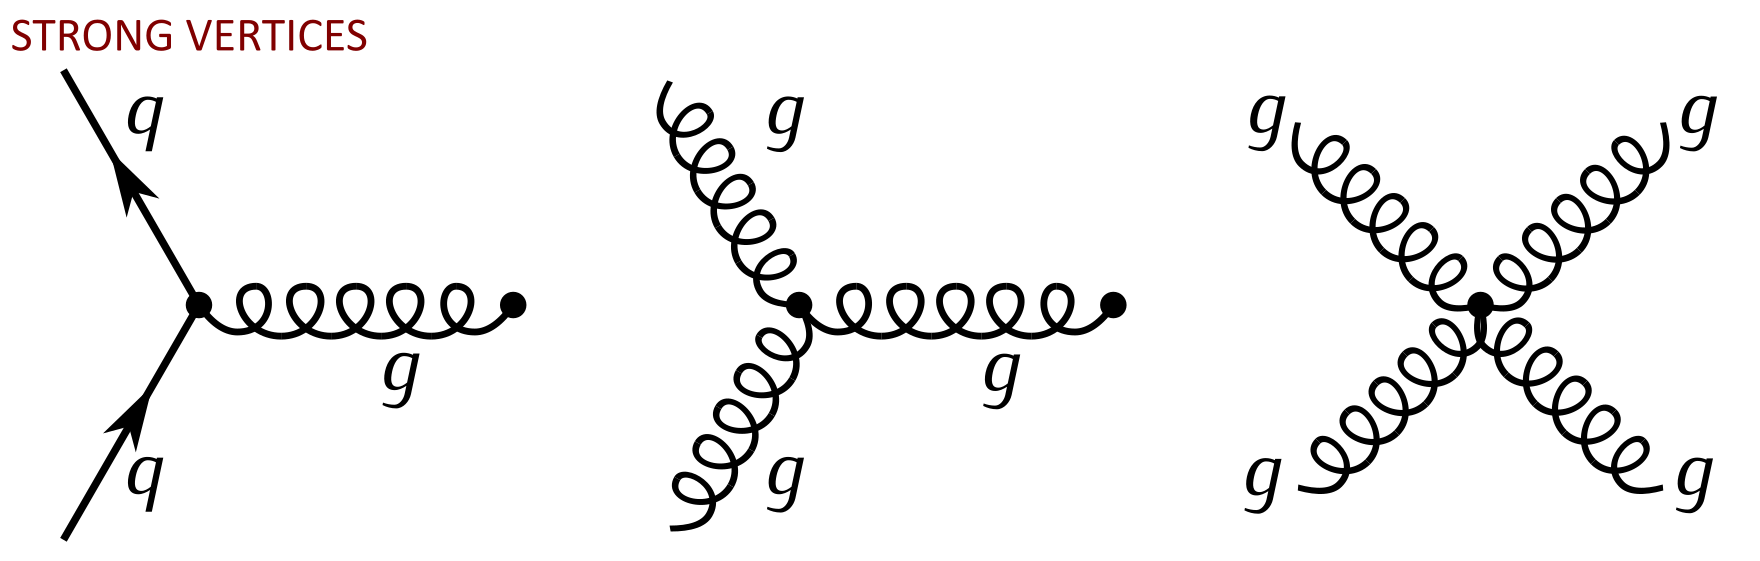
\includegraphics[width=0.5\linewidth,align=c]{pics/SM-Feyn-Strong.png}
\end{equation}
where $q$ is any quark, $g$ is a gluon.
The weak interaction involves the vertices:
\begin{equation}
	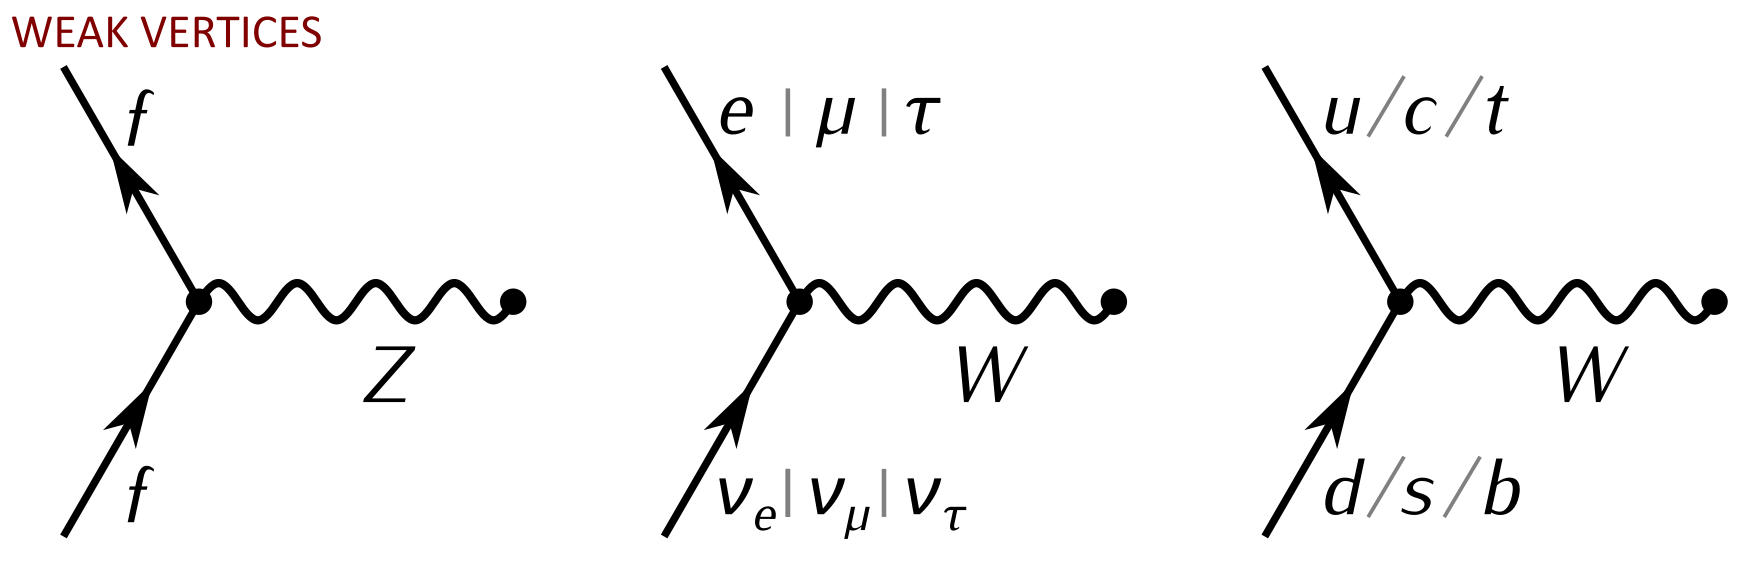
\includegraphics[width=0.5\linewidth,align=c]{pics/SM-Feyn-Weak.png}
\end{equation}
where $f$ is any fermion.

The electro-weak interaction involves the vertices:
\begin{equation}
	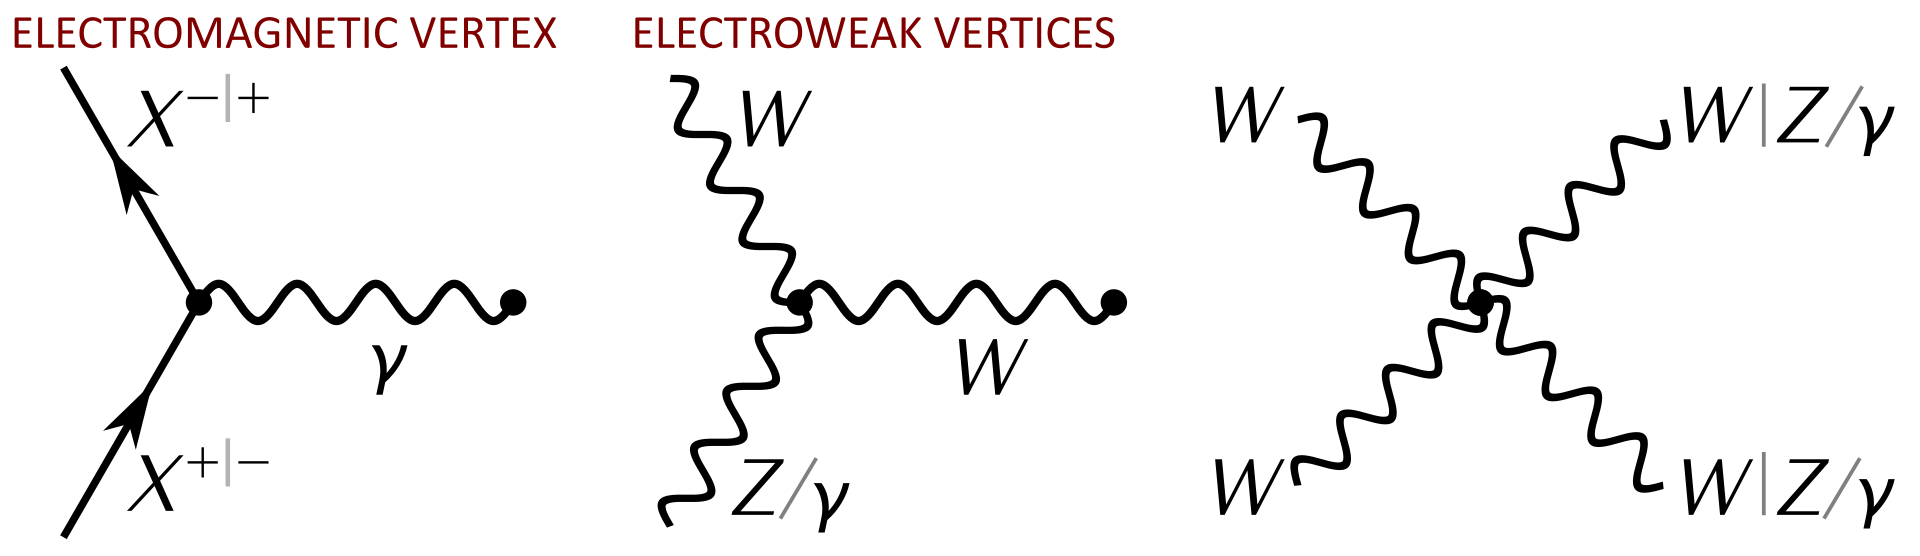
\includegraphics[width=0.5\linewidth,align=c]{pics/SM-Feyn-EW.png}
\end{equation}
where $X$ is any charged particle, $\gamma$ is a photon.
In diagrams with multiple particle labels separated by ``/'', one particle label is chosen. 
In diagrams with particle labels separated by ``|'', the labels must be chosen in the same order. 
For example, in the four boson electroweak case the valid diagrams are WWWW, WWZZ, WW$\gamma\gamma$, WWZ$\gamma$.

The Higgs vertices are:
\begin{equation}
	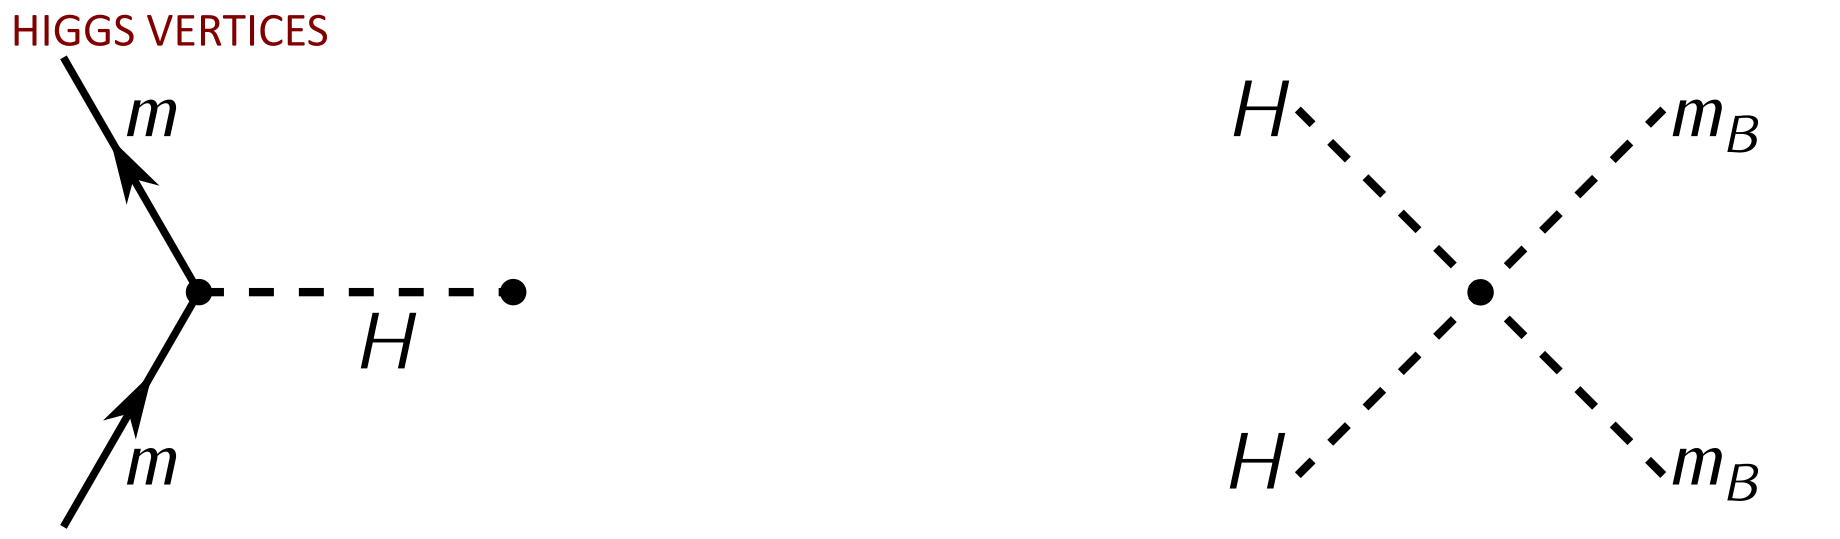
\includegraphics[width=0.5\linewidth,align=c]{pics/SM-Feyn-Higgs.png}
\end{equation}
where $m$ is any particle with mass, $m_B$ is any boson with mass. 
 








\section{Electroweak Interaction}

\subsection{Spontaneous Symmetry Breaking of Higgs Field}
Beside the quarks, leptons and gauge bosons, a doublet scalar field (Higgs) is also introduced in order to generate mass for the particles:
\begin{equation}
	\varphi \equiv \left[\begin{array}{c}
		\varphi_1 \\ \varphi_2
	\end{array} \right],
\end{equation}
which is also an isospin doublet with hyperchage $Y=\frac{1}{2}I$:
\begin{equation}
	\begin{tabular}{c c c c}
		\hline 
		Field & $I_3$ & $Y$ & $q$\\ \hline
		$\varphi_1$ & $1/2$ & $1/2$ & $1$ \\ 
		$\varphi_2$ & $-1/2$ & $1/2$ & $0$ \\  
		\hline 
	\end{tabular}
\end{equation}

The Lagrangian of the Higgs field is 
\begin{equation}\label{eq:SM-Higgs-L1}
	\mathcal L = -\frac{1}{4}(W^a_{\mu\nu})^2 - \frac{1}{4}B_{\mu\nu}^2 +(D^\mu \varphi)^\dagger D_\mu \varphi- V(\varphi),
\end{equation}
where the field strength tensors are
\begin{equation}
\begin{aligned}
	W^a_{\mu\nu} &= \partial_\mu W_\nu^1 - \partial_\nu W^1_\mu + g_2 (W_\mu^2 W_\nu^3 - W_\mu^3 W_\nu^2), \\
	W^a_{\mu\nu} &= \partial_\mu W_\nu^1 - \partial_\nu W^1_\mu + g_2 (W_\mu^3 W_\nu^1 - W_\mu^1 W_\nu^3), \\
	W^a_{\mu\nu} &= \partial_\mu W_\nu^1 - \partial_\nu W^1_\mu + g_2 (W_\mu^1 W_\nu^2 - W_\mu^2 W_\nu^1), \\
	B^a_{\mu\nu} &= \partial_\mu B_\nu^1 - \partial_\nu B^1_\mu,
\end{aligned}
\end{equation}
and the Higgs interaction is
\begin{equation}
	V(\varphi) = \frac{\lambda}{4} \left(\varphi^\dagger \varphi - \frac{v^2}{2} \right)^2.
\end{equation}
This potential gives $\varphi$ a nonzero vacuum expectation value (VEV). 
We can make a gauge transformation so that
\begin{equation}
	\varphi_0 = \langle 0| \varphi |0\rangle = \frac{v}{\sqrt 2} \left[\begin{array}{c}
		0 \\ 1	\end{array} \right].
\end{equation}


The kinetic Lagrangian is described by the SU(2) gauge-invariant Lagrangian
\begin{equation}
	\mathcal L_{\mathrm{kin}} = (D^\mu \varphi)^\dagger D_\mu \varphi,
\end{equation}
where the covariant derivative is
\begin{equation}
	D_\mu = \partial_\mu -i \left(g_1 B_\mu Y + g_2 W^a_\mu T_2^a\right).
\end{equation}
We can introducing the Weinberg angle
\begin{equation}
	\theta_W \equiv\arctan \frac{g_1}{g_2},
\end{equation}
and the fields
\begin{equation}
\begin{aligned}
	W_\mu^\pm &\equiv \frac{1}{\sqrt 2}(W^1_\mu \mp i A_\mu^2), \\
	Z_\mu &\equiv \cos{\theta_W} W^3_\mu - \sin{\theta_W} B_\mu, \\
	A_\mu &\equiv \sin{\theta_W} W_\mu^3 + \cos{\theta_W} B_\mu.
\end{aligned}
\end{equation}
The reverse transformation for $W_\mu^3$ and $B_\mu$ is
\begin{equation}
\begin{aligned}
	W_\mu^3 &= \cos{\theta_W} Z_\mu + \sin{\theta_W} A_\mu, \\
	B_\mu &= -\sin{\theta_W} Z_\mu +\cos{\theta_W} A_\mu.
\end{aligned}
\end{equation}
The off-diagonal part of the Lie algebra becomes
\begin{equation}
	\frac{1}{\sqrt 2}\begin{bmatrix}
		0 &  W^+_\mu \\
		W_\mu^- & 0
	\end{bmatrix},
\end{equation}
and the diagonal part becomes
\begin{equation}
\begin{aligned}
	g_2 W_\mu^3 T^z_2 + g_1 B_\mu Y
	&= g_2 (\cos{\theta_W} Z_\mu + \sin{\theta_W} A_\mu) T^3_2 + g_1 Y (-\sin{\theta_W} Z_\mu +\cos{\theta_W} A_\mu) \\
	&= g_2 \cos{\theta_W} A_\mu \left(T^3_2 + Y\right) + eZ_\mu \left(\cot{\theta_W}T_2^3 - \tan{\theta_W}Y \right) \\
	&= e A_\mu q + \frac{e}{\sin{\theta_W}\cos{\theta_W}} Z_\mu \left(\cos^2{\theta_W}T_2^3 - \sin^2{\theta_W} Y\right) \\
	&= e A_\mu q + \frac{e}{\sin{\theta_W}\cos{\theta_W}} Z_\mu \left(T_2^3 - \sin^2{\theta_W} q\right).
\end{aligned}
\end{equation}
Note that the gauge field $A_\mu$ describe QED, so we identify the coupling constant with the electric charge:
\begin{equation}
	e = g_2 \sin{\theta_W} = g_1 \cos{\theta_W}.
\end{equation}

For Higgs field, 
\begin{equation}
	T^3_2 = \frac{1}{2}\sigma^z, \quad
	Y = \frac{1}{2} I,\quad 
	q = \begin{bmatrix}
		1 & 0 \\ 0 & 0
	\end{bmatrix}.
\end{equation}
$T^3_2 = \frac{1}{2}\sigma^z$, $Y=\frac{1}{2}I$, so 
With the new definition of the field, the Lie algebra of becomes
\begin{equation}
\begin{aligned}
	g_2 W^a_\mu T_2^a + g_1 B_\mu Y 
	&= \frac{e}{2 \sin{\theta_W}} 
	\begin{bmatrix}
		2\sin{\theta_W} A_\mu + \frac{\cos{2\theta_W}}{\cos{\theta_W}} Z_\mu & \sqrt{2} W^+_\mu \\
		\sqrt{2} W_\mu^- & \frac{1}{\cos{\theta_W}} Z_\mu
	\end{bmatrix}.
\end{aligned}
\end{equation}
We can now expand the kinetic term to get the effective mass of the the gauge field in unitary gauge. 
The mass term is the quadratic part of $\varphi$:
\begin{equation}
\begin{aligned}
	\mathcal L_{\mathrm{mass}} 
	&= \varphi_0^\dagger \left(g_2 W^a_\mu T_2^a + g_1 B_\mu Y\right)^2 \varphi_0 \\
	&= \frac{e^2v^2}{8 \sin^2{\theta_W}} 
	\begin{bmatrix}
		0 & 1
	\end{bmatrix} 
	\begin{bmatrix}
		\cdots & \sqrt{2} W^+_\mu \\
		\sqrt{2} W_\mu^- & \frac{1}{\cos{\theta_W}} Z_\mu
	\end{bmatrix}^2
	\begin{bmatrix}
		0 \\ 1
	\end{bmatrix} \\
	&= m_W W^{+\mu} W_\mu^- + \frac{1}{2}m_Z^2 Z^\mu Z_\mu,
\end{aligned}
\end{equation}
where the mass for $W$ and $Z$ bosons are
\begin{equation}
	m_W = \frac{ev}{2 \sin{\theta_W}}, \quad 
	m_Z = \frac{e v}{2\sin{\theta_W}\cos{\theta_W}} = \frac{m_W}{\cos{\theta_W}}.
\end{equation}
Note that the photon field $A_\mu$ does not obtain mass from the Higgs field.



\subsection{Lagrangian of Higgs-Gauge Sector}
We are now going to express the Lagrangian (\ref{eq:SM-Higgs-L1}) in terms of the fields we have just introduced.
In the unitary gauge, the Higgs field can be written as
\begin{equation}
	\varphi = \frac{1}{\sqrt 2} \begin{bmatrix}
		v + H(x) \\ 0
	\end{bmatrix},
\end{equation}
where $H(x)$ is a real scalar field.
The interaction terms gives
\begin{equation}
\begin{aligned}
	V(H) &= \frac{\lambda v^2}{4} H^2 + \frac{\lambda v}{4}H^3 + \frac{\lambda}{16}H^4 \\
	&= \frac{1}{2}m_H^2 H^2 + \frac{m_H^2}{2v} H^3 + \frac{m_H^2}{8v^2}H^4,
\end{aligned} 
\end{equation}
where we have defined the Higgs mass
\begin{equation}
	m_H^2 = \frac{\lambda v^2}{2}.
\end{equation}
Also, the fluctuation around the $\varphi_0$ also create coupling between Higgs field and the gauge fields.
We can simply replace $v^2$ with $(v+H)^2$ in the gauge field mass term to capture the coupling.
Thus, the Lagrangian is
\begin{equation}
	\mathcal L_{\mathrm{H}} = \partial^\mu H^\dagger \partial_\mu H - V(H) + \left(m_W W^{+\mu} W_\mu^- + \frac{1}{2}m_Z^2 Z^\mu Z_\mu \right) \left(H^2+2vH \right).
\end{equation}
Now consider the Lagrangian for the gauge field
\begin{equation}
	\mathcal L_\mathrm{W} = -\frac{1}{4}(W^a_{\mu\nu})^2 - \frac{1}{4}B_{\mu\nu}^2 + m_W W^{+\mu} W_\mu^- + \frac{1}{2}m_Z^2 Z^\mu Z_\mu.
\end{equation}
We can regroup the field strength as
\begin{equation}
\begin{aligned}
	W^+_{\mu\nu} &= D_\mu W_\nu^+ - D_\nu W^+_\mu, \\
	W^-_{\mu\nu} &= D_\mu^\dagger W_\nu^- - D_\nu^\dagger W^-_\mu, \\
	W^3_{\mu\nu} &= \sin{\theta_W} F_{\mu\nu} + \cos{\theta_W}Z_{\mu\nu} -ig_2(W^+_\mu W^-_\nu - W_\mu^- W_\nu^+), \\
	B^a_{\mu\nu} &= \cos{\theta_W} F_{\mu\nu} - \sin{\theta_W} Z_{\mu\nu},
\end{aligned}
\end{equation}
where we have defined 
\begin{equation}
\begin{aligned}
	W^\pm_{\mu\nu} &= \frac{1}{\sqrt 2} (W^1_{\mu\nu} \mp i W^2_{\mu\nu}), \\
	F_{\mu\nu} &= \partial_\mu A_\nu - \partial_\nu A_\mu, \\
	Z_{\mu\nu} &= \partial_\mu Z_\nu - \partial_\nu Z_\mu.
\end{aligned}
\end{equation}
The covariant derivative for $W^\pm$ field is
\begin{equation}
\begin{aligned}
	D_\mu &= \partial_\mu -i g_2 W^3_\mu \\
	&= \partial_\mu -i g_2 \left(\sin{\theta_W}A_\mu + \cos{\theta_W} Z_\mu \right) \\
	&= \partial_\mu -i e \left(A_\mu + \cot{\theta_W} Z_\mu \right)
\end{aligned}
\end{equation}
So the Lagrangian for the gauge field is
\begin{equation}
\begin{aligned}
	\mathcal L_\mathrm{W}
	=&\ -\frac{1}{4}(2W_{\mu\nu}^+ W^{-\mu\nu} + W_{\mu\nu}^3 W^{3\mu\nu}) -\frac{1}{4} B_{\mu\nu}B^{\mu\nu} + m_W W^{+\mu} W_\mu^- + \frac{1}{2}m_Z^2 Z^\mu Z_\mu \\
	=&\ -\frac{1}{4}(F_{\mu\nu}F^{\mu\nu} + Z_{\mu\nu} Z^{\mu\nu}) - D^{\mu} W^{+\nu} D^\dagger_\mu W_\nu^- + D^\mu W^{+\nu} D^\dagger_\nu W^-_\mu \\
	&\ +ie (F^{\mu\nu} + \cot{\theta_W} Z^{\mu\nu})W_\mu^+ W_\nu^- + m_W W^{+\mu} W_\mu^- + \frac{1}{2}m_Z^2 Z^\mu Z_\mu \\
	&\ -\frac{e^2}{2\sin^2{\theta_W}} \left(W^{+\mu}W^-_\mu W^{+\nu}W^-_\nu - W^{+\mu}W^+_\mu W^{-\nu}W^-_\nu \right).
\end{aligned}
\end{equation}
We remark that in the unitary gauge, there is no redundancy of the gauge field.
No ghost field is needed in the quantization procedure.


\section{Yukawa Couplings}
The fermion fields in the electroweak interaction
\begin{equation}
	\begin{tabular}{c c c c}
		\hline 
		Field & $I_3$ & $Y$ & $q$\\ \hline
		$u_L$ & $1/2$ & $1/6$ & $2/3$ \\ 
		$d_L$ & $-1/2$ & $1/6$ & $-1/3$ \\  
		$u_R$ & $0$ & $2/3$ & $2/3$ \\
		$d_R$ & $0$ & $-1/3$ & $-1/3$ \\ \hline
		$e_L$ & $-1/2$ & $-1/2$ & $-1$ \\ 
		$\nu_{eL}$ & $1/2$ & $-1/2$ & $0$ \\  
		$e_R$ & $0$ & $-1$ & $-1$ \\
		$\nu_{eR}$ & $0$ & $0$ & $0$ \\
		\hline 
	\end{tabular}
\end{equation}

The kinetic term for the fermion Lagrangian is
\begin{equation}
\begin{aligned}
	\mathcal L_{\mathrm{kin}}
	=&\ i Q^\dagger_J \sigma^\mu D_\mu Q_J + i u_{RJ}^\dagger \bar\sigma^\mu D_\mu u_{RJ} + i d_{RJ}^\dagger \bar\sigma^\mu D_\mu d_{RJ} \\
	& + i L^\dagger_J \sigma^\mu D_\mu L_J + i e_{RJ}^\dagger \bar\sigma^\mu D_\mu e_{RJ} + i \nu_{RJ}^\dagger \bar\sigma^\mu D_\mu \nu_{RJ},
\end{aligned}
\end{equation}
where we have use the index $J$ to label the generation of the fermion:
\begin{equation}
\begin{aligned}
	u_{RJ} &= \{u_R, c_R, t_R\}, & 
	d_{RJ} &= \{d_R, s_R, b_R\}, \\
	e_{RJ} &= \{e_R, \mu_R, \tau_R\}, &
	\nu_{RJ} &= \{\nu_{eR},\nu_{\mu R},\nu_{\tau R}\}.
\end{aligned}
\end{equation}

The left-handed SU(2) gauge symmetry forbid any fermion mass term, which is incompatible with the reality.
However, fermion can obtain fermion mass by introducing Yukawa coupling between the Higgs and fermion fields.

\subsection{Quark Sector}
The Yukawa coupling between quark and Higgs is
\begin{equation}
	\mathcal L_{q,\mathrm{Yuk}}
	= - \varepsilon^{ij} Y^u_{IJ} Q^\dagger_{iI} \varphi^\dagger_j u_{RJ}
	- Y^d_{IJ} Q^\dagger_{I} \varphi d_{RJ} +h.c..
\end{equation}
The first term corresponds to
\begin{equation}
	\left(\bar 3, \bar 2, -\frac{1}{6}\right) \times \left(1, \bar 2, -\frac{1}{2}\right) \times \left(3, 1, \frac{2}{3}\right) = \left(1,1,0\right)\oplus \cdots,
\end{equation}
with $\varepsilon^{ij}$ being the Clebsch-Gordan coefficient, and the second term corresponds to
\begin{equation}
	\left(\bar 3, \bar 2, -\frac{1}{6}\right) \times \left(1, 2, \frac{1}{2}\right) \times \left(3, 1, -\frac{1}{3}\right) = \left(1,1,0\right).
\end{equation}
Now substitute $\varphi$ with 
\begin{equation}
	\varphi = \frac{1}{\sqrt 2} \begin{bmatrix}
		0 \\ v+H
	\end{bmatrix}.
\end{equation}
The Yukawa potential then gives quark mass term:
\begin{equation}
	\mathcal L_{Q,\mathrm{Yuk}}
	= -\frac{v+H}{\sqrt 2} \left( Y^u_{IJ} u^\dagger_{LI} u_{RJ} +Y^d_{IJ} d^\dagger_{LI} d_{RJ} \right) +h.c..
\end{equation}
We can then use a basis transformation (singular value decomposition) to diagonalize the coupling matrix:
\begin{equation}
	Y^u_{IJ} = U_u M_u K^\dagger_u, \quad
	Y^d_{IJ} = U_d M_d K^\dagger_d,
\end{equation}
where $M_u$ and $M_d$ are diagonal matrices.
We can change the basis
\begin{equation}
\begin{aligned}
	u_L &\rightarrow U_u u_L, & u_R &\rightarrow K_u u_R, \\
	d_L &\rightarrow U_d d_L, & d_R &\rightarrow K_d d_R,
\end{aligned}
\end{equation}
and define the diagonal masses:
\begin{equation}
	m_{u_I} = \frac{v}{\sqrt 2} (M_u)_{II}, \quad 
	m_{d_I} = \frac{v}{\sqrt 2} (M_d)_{II},
\end{equation}
then the Lagrangian in the quark sector can be expressed as:
\begin{equation}
\begin{aligned}
	\mathcal L_Q =&\ \sum_I \bar u_I\left(i\cancel D^c-m_{u_I}\right)u_I + \sum_I \bar d_I \left(i \cancel D^c-m_{d_I}\right)d_I \\
	& -\frac{H}{v} \sum_I\left(m_{u_I}\bar u_I u_I+m_{d_I}\bar d_I d_I \right) + \mathcal L_{Q-G},
\end{aligned}
\end{equation}
where $\cancel D^c$ is the covariant derivative in QCD (neglecting the electroweak gauge), and $\mathcal L_{Q-G}$ denotes the coupling between quarks and the gauge fields.
Using the expression of the Lie algebra
\begin{equation}
\begin{aligned}
	g_2 \sum_{a=1}^2 W^a_\mu T^a_2 &= \frac{e}{\sqrt{2}\sin{\theta_W}}\begin{bmatrix}
		0 & W_\mu^+ \\ W_\mu^- & 0
	\end{bmatrix}, \\
	g_2 W_\mu^3 T^z_2 + g_1 B_\mu Y
	&= e A_\mu q + \frac{e}{\sin{\theta_W}\cos{\theta_W}} Z_\mu \left(T_2^3 - \sin^2{\theta_W} q\right),
\end{aligned}
\end{equation}
The gauge-current coupling is:
\begin{equation}
	\mathcal L_{Q-G} = \frac{e}{\sqrt{2}\sin{\theta_W}} \left(W^{+}_\mu J_Q^{+\mu} + W^{-}_\mu J_Q^{-\mu} \right) + e A_\mu J^{\mu}_{\mathrm{EM},Q} + \frac{e}{\sin{\theta_W}\cos{\theta_W}} Z_\mu J^\mu_{z,Q},
\end{equation}
where the currents are defined as
\begin{equation}
\begin{aligned}
	J^{+\mu}_Q &= d_{LI}^\dagger \bar\sigma^\mu u_{LI}, \quad
	J^{-\mu}_Q = u_{LI}^\dagger \bar\sigma^\mu d_{LI}, \\
	J^\mu_{\mathrm{EM},Q} &= \frac{2}{3} u_{LI}^\dagger \bar\sigma^\mu u_{LI} - \frac{1}{3} d_{LI}^\dagger \bar\sigma^\mu d_{LI}, \\
	J_{z,Q}^\mu &= \frac{1}{2} u_{LI}^\dagger \bar\sigma^\mu u_{LI} - \frac{1}{2} d_{LI}^\dagger \bar\sigma^\mu d_{LI} J^\mu_3-\sin^2{\theta_W}J_{\mathrm{EM},Q}^\mu.
\end{aligned}
\end{equation}
We note that in the definition of the currents, the quarks is the eigenstates of the weak interaction, not the mass eigenstates.
If we define the quarks as the particle with definite mass, the above definition shall be rotation by a unitary matrix.


\subsection{Lepton Sector}
The coupling between Higgs and $e_R$ has the general Yukawa form:
\begin{equation}
	\mathcal L_{e,\mathrm{Yuk}} = -Y^e_{IJ} L_{iI}^\dagger \varphi_j e_{R iJ} + h.c.,
\end{equation}
where $y_{IJ}$ is the Hermitian coupling matrix on generation space.
The Yukawa coupling term corresponds to
\begin{equation}
	\left(\bar 2, \frac{1}{2}\right) \times \left(2, \frac{1}{2}\right) \times \left(1, -1\right) = \left(1,0\right),
\end{equation}
which is indeed a singlet under gauge transformation (it is also a singlet under Lorentz transformation).
The Higgs field then produce the term
\begin{equation}
	\mathcal L_{e,\mathrm{Yuk}} = -\frac{Y^e_{IJ}}{\sqrt 2}(v+H) e_{LI}^\dagger e_{RJ} + h.c.,
\end{equation}
We then diagonalize the coupling matrix:
\begin{equation}
	 Y^e_{IJ} = \left[U_{e} M_e K^\dagger_{e}\right]_{IJ},
\end{equation}
where $M_e$ is diagonal.
We can then change the basis by
\begin{equation}
\begin{aligned}
	e_R &\rightarrow K_e e_R, \\
	e_L &\rightarrow U_e e_L,
\end{aligned}
\end{equation}
Then the coupling gives the mass:
\begin{equation}
	\mathcal L_{e,\mathrm{Yuk}} 
	= - \sum_I m_{e_I} \bar e_I e_I - \frac{H}{v}\sum_I m_{e_I} \bar e_I e_I,
\end{equation}
where
\begin{equation}
	m_{e_I} = \frac{v}{\sqrt 2} (M_e)_{II}.
\end{equation}

Now we consider the neutrino mass, which is much smaller than electrons.
The neutrinos can similarly obtain mass by coupling to Higgs field.
However, as the neutrinos being charge neutral, the mass term can come from Yukawa coupling as well as the Majorana pairing:
\begin{equation}
\begin{aligned}
	\mathcal L_{\nu,\mathrm{Yuk}} 
	&= - Y^\nu_{IJ} \varepsilon^{ij} L_{iI} \varphi_j \nu_{RJ} - \frac{1}{2} M_{IJ} \nu_{RI} \cdot \nu_{RJ} + h.c. \\
	&= -\frac{Y^\nu_{IJ}}{\sqrt 2}(v+H) \nu_{LI}^\dagger \nu_{RJ} - \frac{1}{2}M_{IJ}\nu_{RI}\cdot \nu_{RJ} + h.c.
\end{aligned}
\end{equation}
The first term corresponds to
\begin{equation}
	\left(2, -\frac{1}{2}\right) \times \left(2, \frac{1}{2}\right) \times \left(1, 0\right) = \left(1,0\right) \oplus(3,0),
\end{equation}
and $\varepsilon^{ij}$ is the Clebsch-Gordan coefficients.
The second term is automatically a gauge singlet.
We can make a basis change to make $Y$ diagonal, and define a new set of Dirac spinors from single Weyl spinors:
\begin{equation}
	\psi_1 = \begin{pmatrix}
		\nu_L \\ i\sigma^2 \nu_L^*
	\end{pmatrix}, \quad
	\psi_2 = \begin{pmatrix}
		-i\sigma^2 \nu_R^* \\ \nu_R
	\end{pmatrix},
\end{equation}
and the effective mass term can be written as:
\begin{equation}
	\mathcal L_{\nu,\mathrm{mass}} 
	= -\sum_I \frac{Y_{II} v}{\sqrt 2}\bar\psi_{1I} \psi_{2I} - \sum_{IJ}\frac{1}{2} M_{IJ} \bar\psi_{2I} \psi_{2J}.
\end{equation}
Now the Dirac spinor $\psi_1$ and $\psi_2$ can mix, and a suitable mixing renders the mass term diagonal.
If $M \gg m$, the eigenvalues of the mass term will be a huge masses plus some tiny masses.
In general, the low-energy part of the mass term is
\begin{equation}
	\mathcal L_{\nu,\mathrm{mass}} = -\sum_I m_{\nu_I}\bar\nu_I \nu_I \left(1+\frac{H}{v}\right)^2,
\end{equation}

With the discussion above, we can write down the Lagrangian in the lepton sector:
\begin{equation}
\begin{aligned}
	\mathcal L_L =&\ \sum_I \bar e_I (i\cancel\partial-m_{e_I})e_I + \sum_I \nu_{LI}^\dagger (\bar\sigma^\mu \partial_\mu -m_{\nu_I})\nu_{LI} \\
	& -\frac{H}{v} \sum_I \left(m_{e_I} \bar e_I e_I + m_{\nu_I}\bar\nu_{LI}\nu_{LI}\right)+ \mathcal L_{L-G},
\end{aligned}
\end{equation}
where $\mathcal L_{L-G}$ is the lepton-gauge coupling term:
\begin{equation}
	\mathcal L_{L-G} = \frac{e}{\sqrt{2}\sin{\theta_W}}\left(W^{+}_\mu J_L^{+\mu} + W^{-}_\mu J_L^{-\mu} \right) + e A_\mu J^{\mu}_{\mathrm{EM},L} + \frac{e}{\sin{\theta_W}\cos{\theta_W}} Z_\mu J^\mu_{z,L},
\end{equation}
where the current is defined as 
\begin{equation}
\begin{aligned}
	J^{+\mu}_L &= e_{LI}^\dagger \bar\sigma^\mu \nu_{LJ}, \\
	J^{-\mu}_L &= \nu_{LI}^\dagger \bar\sigma^\mu e_{LJ}, \\
	J^\mu_{\mathrm{EM},L} &= - e_{LI}^\dagger \bar\sigma^\mu e_{LI} \\
	J_{z,L}^\mu &= \frac{1}{2} \nu_{LI}^\dagger \bar\sigma^\mu \nu_{LI} - \frac{1}{2} e_{LI}^\dagger \bar\sigma^\mu e_{LI} J^\mu_3-\sin^2{\theta_W}J_{\mathrm{EM},L}^\mu.
\end{aligned}
\end{equation}
We note that although right-handed neutrinos are introduced, experimentally we can only directly observe the left-handed neutrinos.
For the same reason the eigenstate of the weak interaction works more natural than the mass eigenstate for neutrinos. 
We choose to define the neutrinos as what we directly measured -- the left-handed ``particle'' with no definite mass.



\subsection{Particle Mixing}

\subsubsection{Quark Mixing}
In the above discussion, when talking about ``particles'', we actually mean two different things. 
The original definition of the particle is an excitation with definite energy.
But in the weak interaction process, say
\begin{equation}
	u \rightarrow d + W^+,
\end{equation}
the strange and charm quark is the eigenstate of the weak interaction.
That is, the weak interaction can change a state called $u$ to a states called $d$, both of which not necessarily have fixed energies.
If we stick to the original definition of the particles, it turns out that the isospin doublet $Q_I$ we have just defined is not exact.
It really should be written as
\begin{equation}
	Q_I = \left[
		\begin{pmatrix} u_L' \\ d_L' \end{pmatrix},
		\begin{pmatrix} c_L' \\ s_L' \end{pmatrix},
		\begin{pmatrix} t_L' \\ b_L' \end{pmatrix}
	\right],
\end{equation}
where the primed quarks are mixtures of particle quarks from three generations.
Without the loss of generality, we can identify $u'=u$, $c'=c$, $t'=t$, the mixing of quarks happens for the remaining three flavors:
\begin{equation}
	\begin{pmatrix}
		d' \\ s' \\ b'
	\end{pmatrix}
	= \begin{bmatrix}
		V_{ud} & V_{us} & V_{ub} \\
		V_{cd} & V_{cs} & V_{cb} \\
		V_{td} & V_{ts} & V_{tb}
	\end{bmatrix}
	\begin{pmatrix}
		d \\ s \\ b.
	\end{pmatrix}
\end{equation}
The matrix $V$, being unitary, is called the \textit{Cabbibo-Kobayashi-Maskawa} (CKM) matrix.
From the calculation above, we know
\begin{equation}
	V \equiv U^\dagger_u U_d.
\end{equation}
The quark mixing changes the original definition of $J^\pm_Q$ to:
\begin{equation}
\begin{aligned}
	J^{+\mu}_Q &= {d'}_{LI}^{\dagger} \bar\sigma^\mu u_{LI}
		= V^\dagger_{IJ} d_{LI}^\dagger \bar\sigma^\mu u_{LJ}, \\
	J^{-\mu}_Q &= u_{LI}^\dagger \bar\sigma^\mu d'_{LI}
		= V_{IJ} u_{LI}^\dagger \bar\sigma^\mu d_{LJ}.
\end{aligned}
\end{equation}
Note that the diagonal current $J_{\mathrm{EM}}$ or $J_z$ will not change change under the basis transformation.

The experimental value of the CKM matrix is approximately
\begin{equation}
	\begin{bmatrix}
		\left|V_{u d}\right| & \left|V_{u s}\right| & \left|V_{u b}\right| \\
		\left|V_{c d}\right| & \left|V_{c s}\right| & \left|V_{c b}\right| \\
		\left|V_{t d}\right| & \left|V_{t s}\right| & \left|V_{t b}\right|
	\end{bmatrix} =
	\begin{bmatrix}
		0.97 & 0.22 & 0.004 \\
		0.22 & 0.97 & 0.04 \\
		0.009 & 0.04 & 0.999
	\end{bmatrix}.
\end{equation}
We see the CKM matrix is closed to an identity matrix, and the most mixing happens between $d$ and $s$ quarks, i.e.,
\begin{equation}
\begin{aligned}
	d' &= \cos\theta_c\ d + \sin\theta_c\ s \\
	s' &= -\sin\theta_c\ d + \cos\theta_c\ s.
\end{aligned}
\end{equation}
Here the angle $\theta_c \approx 13^{\circ}$ is called the Cabbibo angle.
It correct the quark decay process to:
\begin{equation}
	\left[u \rightarrow d' + W^+\right]
	= \cos\theta_c \left[u \rightarrow d + W^+\right] + \sin\theta_c \left[u \rightarrow s + W^+\right].
\end{equation}


\subsubsection{Neutrino Oscillation}
Quite similarly, particles in lepton sector also mix.
We choose to identify $e'_L = e_L$ (similarly for muon and tauon).
Neutrinos that have specific mass are called $\nu_1$, $\nu_2$, and $\nu_3$ instead, which satisfies
\begin{equation}
	\begin{pmatrix}
		\nu_{e} \\ \nu_{\mu} \\ \nu_{\tau}
	\end{pmatrix} = 
	\begin{bmatrix}
		U_{e 1} & U_{e 2} & U_{e 3} \\
		U_{\mu 1} & U_{\mu 2} & U_{\mu 3} \\
		U_{\tau 1} & U_{\tau 2} & U_{\tau 3}
	\end{bmatrix}
	\begin{pmatrix}
		\nu_{1} \\ \nu_{2} \\ \nu_{3}
	\end{pmatrix},
\end{equation}
the $3 \times 3$ matrix is known as the \textit{Pontecorvo-Maki-Nakagawa-Sakata} (PMNS) matrix, or simply the neutrino mixing matrix.
Its value is roughly
\begin{equation}
	\begin{bmatrix}
		\left|U_{e 1}\right|\left|U_{e 2}\right|\left|U_{e 3}\right| \\
		\left|U_{\mu 1}\right|\left|U_{\mu 2}\right|\left|U_{\mu 3}\right| \\
		\left|U_{\tau 1}\right|\left|U_{\tau 2}\right|\left|U_{\tau 3}\right|
	\end{bmatrix} \approx
	\begin{bmatrix}
		0.8 & 0.5 & 0.1 \\
		0.3 & 0.5 & 0.7 \\
		0.4 & 0.6 & 0.6
	\end{bmatrix}.
\end{equation}
The neutrino mixing means that in the weak process, say
\begin{equation}
	e \rightarrow \nu_e + W^-,
\end{equation}
the produced neutrino $\nu_e$ is not an energy eigenstate of the SM Hamiltonian -- it will oscillates.
As for the definition of the lepton current $J^\pm_L$. 
If we stick to the definition of neutrino as the eigenstate of the weak interaction -- since that is what we get from the particle decay process -- we do not need to change the definition, but we should remember that such ``neutrinos'' do not have fixed mass.


\subsection{Restore 4-Fermion Theory}
Finally, we can sum over the current, and write down the total fermion-gauge coupling:
\begin{equation}
	\mathcal L_{F-G} = \frac{e}{\sqrt{2}\sin{\theta_W}} \left(W^{+}_\mu J^{+\mu} + W^{-}_\mu J^{-\mu} \right) + e A_\mu J^{\mu}_{\mathrm{EM}} + \frac{e}{\sin{\theta_W}\cos{\theta_W}} Z_\mu J^\mu_{z}.
\end{equation}
From the current-gauge coupling, we can recover the effective 4-fermion theory by integrating out the gauge field.
In the low energy regime ($p^2 \ll m_W^2$), the vertex function for electron decay is:
\begin{equation}
	2\left(\frac{e}{\sqrt{2}\sin{\theta_W}} \right)^2 J^+_\mu \frac{g^{\mu\nu}}{p^2-m_W^2} J^-_\nu 
	\simeq \frac{e^2}{m_W^2 \sin^2{\theta_W}} J^{+\mu} J^-_\mu.
\end{equation}
The diagonal part of the vertex is
\begin{equation}
	\left(\frac{e}{\sin{\theta_W}\cos{\theta_W}} \right)^2 J^z_\mu \frac{g^{\mu\nu}}{p^2-m_Z^2} J^z_\nu 
	\simeq -\frac{e^2}{m_Z^2 \sin^2{\theta_W}\cos^2{\theta_W}} J^{z\mu} J^z_\mu.
\end{equation}\
Note that $m_Z^2\cos^2{\theta_W} = m_W^2$, we can then identify the fermion constant
\begin{equation}
	\frac{4G_F}{\sqrt 2} = \frac{e^2}{m_W^2 \sin^2{\theta_W}},
\end{equation}
and the 4-Fermion vertex is
\begin{equation}
	\mathcal L_{4F} = -\frac{4G_F}{\sqrt 2} \left(J^{+\mu} J_\mu^- + J^{z\mu} J_\mu^z \right).
\end{equation}




















\end{document}


